\newpage
\section{Evaluación del Sistema}
\label{cap:evaluacion_sistema}

La culminación de la fase de despliegue físico da paso a la auditoría técnica del prototipo. En este capítulo se analiza empíricamente el rendimiento del sistema, evaluando la latencia en las comunicaciones y la carga computacional del servidor perimetral, la fiabilidad de las inferencias lógicas del motor de contexto, la eficiencia energética global y el análisis de los riesgos y contingencias operacionales.

\subsection{Análisis técnico y de rendimiento}
\label{sec:rendimiento_tecnico}
El rendimiento temporal de las comunicaciones locales constituye un factor crítico en arquitecturas distribuidas de control y automatización. Se han realizado ensayos cronométricos sistemáticos para cuantificar el retardo o latencia de conmutación de los actuadores del sistema. Para ello, se midió el tiempo transcurrido desde la activación física de una interrupción de entrada (como la separación del interruptor Reed en la puerta) hasta el disparo físico del relé de iluminación a través del servidor central. 

Los resultados medidos en la red local inalámbrica bajo la API nativa de ESPHome se compararon con los tiempos de respuesta típicos ofrecidos por soluciones comerciales basadas en la nube pública (como Tuya Smart o Sonoff/eWeLink en servidores de la región europea). La comparativa obtenida se ilustra en la Figura~\ref{fig:latencia_comparativa}.

\begin{figure}[H]
    \centering
    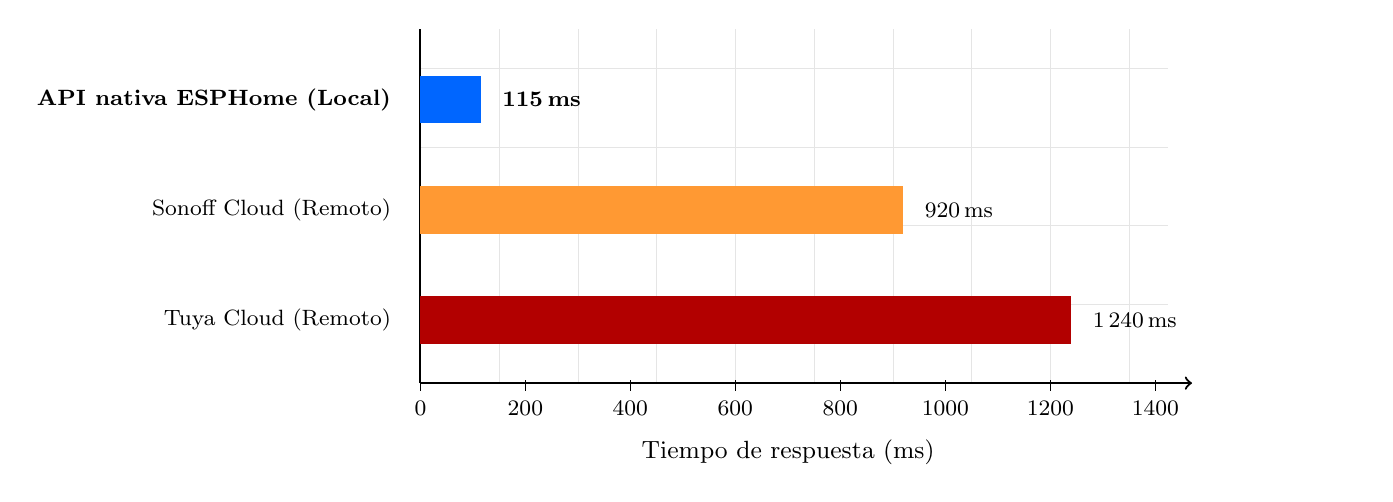
\begin{tikzpicture}
        % Rejilla fina en el área de datos (de 0 a 9.5 cm de ancho)
        \draw[very thin, gray!20, step=1cm] (0,0) grid (9.5,4.5);
        
        % Eje X y ticks sin etiqueta al final
        \draw[->, thick] (0,0) -- (9.8,0);
        \node[anchor=north, font=\small] at (4.67, -0.6) {Tiempo de respuesta (ms)};
        
        \foreach \x in {0,200,400,600,800,1000,1200,1400}
            \draw (\x/150, 1pt) -- (\x/150, -3pt) node[anchor=north, font=\footnotesize] {\x};

        % Eje Y
        \draw[-, thick] (0,0) -- (0,4.5);
        
        % Etiquetas del sistema (alineadas a la derecha, a la izquierda del eje Y)
        \node[anchor=east, font=\footnotesize\bfseries] at (-0.25, 3.6) {API nativa ESPHome (Local)};
        \node[anchor=east, font=\footnotesize] at (-0.25, 2.2) {Sonoff Cloud (Remoto)};
        \node[anchor=east, font=\footnotesize] at (-0.25, 0.8) {Tuya Cloud (Remoto)};
        
        % Barras de datos y valores
        % 1. API Nativa ESPHome (Local) -- 115 ms -> 115/150 = 0.767 cm
        \fill[blue!60!cyan] (0, 3.3) rectangle (115/150, 3.9);
        \node[anchor=west, font=\footnotesize\bfseries] at (115/150 + 0.15, 3.6) {115\,ms};

        % 2. Sonoff/eWeLink Cloud -- 920 ms -> 920/150 = 6.133 cm
        \fill[orange!80!white] (0, 1.9) rectangle (920/150, 2.5);
        \node[anchor=west, font=\footnotesize] at (920/150 + 0.15, 2.2) {920\,ms};

        % 3. Tuya/SmartLife Cloud -- 1240 ms -> 1240/150 = 8.267 cm
        \fill[red!70!black] (0, 0.5) rectangle (1240/150, 1.1);
        \node[anchor=west, font=\footnotesize] at (1240/150 + 0.15, 0.8) {1\,240\,ms};
        
        % Margen invisible a la derecha para recentrar el gráfico (desplazar a la izquierda en la página)
        \path (12.0, 0);
    \end{tikzpicture}
    \caption{Comparativa de la latencia de respuesta en conmutación local mediante la API nativa de ESPHome frente a servidores comerciales remotos en la nube.}
    \label{fig:latencia_comparativa}
\end{figure}

El análisis temporal revela que la API nativa de ESPHome, al operar de forma directa mediante sockets TCP persistentes en red local cableada o inalámbrica (sin intermediarios de red WAN, latencias DNS o saltos de enrutamiento externos), reduce el retardo de conmutación en un factor aproximado de $8$ y $10$ veces frente a los entornos cloud de Sonoff y Tuya, respectivamente. Los 115\,ms de respuesta del prototipo resultan prácticamente imperceptibles para el usuario, garantizando una alta calidad en la ergonomía interactiva.

Por otro lado, se ha evaluado el impacto de la carga computacional en el servidor central (Raspberry Pi 4 con 1\,GB de RAM) durante la monitorización y registro continuado de datos en producción. El uso medio de la unidad central de procesamiento (CPU) se estabilizó sistemáticamente en valores por debajo del 5\,\% debido al carácter estático de las consultas del motor analítico local y a la optimización de los contenedores Docker. 

La memoria de acceso aleatorio (RAM) registró una ocupación media constante de 620\,MB (aproximadamente el 62\,\% de la capacidad física del dispositivo). Esto valida la viabilidad del empleo de un nodo perimetral de bajo coste y prestaciones moderadas para gestionar la lógica contextual de la vivienda de forma sólida e ininterrumpida.

\subsection{Fiabilidad y tolerancia a fallos}
\label{sec:fiabilidad_fallos}
La robustez operacional de la máquina de estados de contexto reside en la tolerancia a fallos del software y la capacidad de absorber lecturas sensoras anómalas. A diferencia de las soluciones basadas en un único transductor físico, el motor lógico del prototipo implementa redundancias cruzadas que blindan el funcionamiento:

\begin{itemize}
    \item \textbf{Fusión sensorial redundante:} en el caso práctico de una lectura errónea o persistencia en nivel bajo del sensor de luminosidad LDR en horas nocturnas (lo que forzaría teóricamente una inferencia permanente del estado \texttt{Durmiendo}), el sistema valida la transición cruzando los datos del radar de ondas milimétricas del Nodo Escritorio. Si el radar no registra presencia absoluta durante el retardo de seguridad paramétrico, la prioridad de iluminación decae y el motor realiza la transición al estado \texttt{Ausente}, evitando la parálisis o el bloqueo lógico del sistema de potencia.
    \item \textbf{Tolerancia a cortes de red e interrupciones de alimentación:} la arquitectura de comunicaciones locales cuenta con un sistema de reintento activo de sincronización de sockets en la API de ESPHome. Ante caídas puntuales del enrutador Wi-Fi o desconexiones eléctricas transitorias de los microcontroladores, cada nodo ESP32 intenta restablecer el canal de socket TCP de forma autónoma. Home Assistant recupera dinámicamente las entidades vinculadas sin requerir un reinicio manual del servidor o de los nodos. Por motivos de seguridad física, las salidas de los relés se configuran mediante el \textit{firmware} en modo apagado persistente (\texttt{restore\_mode: ALWAYS\_OFF}) para evitar la activación involuntaria de cargas eléctricas ante el restablecimiento del flujo de corriente tras un apagón general.
\end{itemize}

\subsection{Pruebas funcionales y validación del motor de automatizaciones}
\label{sec:pruebas_funcionales}

La verificación del comportamiento dinámico de la infraestructura requiere contrastar el funcionamiento del motor lógico y las reglas de gestión centralizada frente a estímulos reales del entorno. Para llevar a cabo esta validación de forma trazable y científica, se ha adoptado como herramienta principal el motor de trazas de ejecución de Home Assistant (\textit{Automation Traces}). Esta funcionalidad del servidor central registra y representa gráficamente el flujo lógico exacto que sigue cada automatización tras ser disparada. En particular, almacena un historial estructurado en formato JSON que detalla:

\begin{itemize}
    \item \textbf{Evento disparador (\textit{Trigger}):} la entidad y cambio de estado específico que inició la evaluación.
    \item \textbf{Caminos de decisión (\textit{Conditions}):} el resultado binario (verdadero/falso) obtenido al evaluar cada una de las variables condicionales y de fusión de sensores.
    \item \textbf{Acciones ejecutadas (\textit{Actions}):} la secuencia cronológica de órdenes de control transmitidas a los actuadores físicos a través del canal de comunicación local.
    \item \textbf{Tiempos de cómputo y latencias internas:} la marca temporal exacta de cada transición de la secuencia, lo que permite auditar retardos internos.
\end{itemize}

A continuación, se define la batería de casos de prueba funcionales diseñados para validar los escenarios lógicos esenciales descritos en el modelado del sistema (Sección~\ref{sec:modelado_logico}). Cada caso de prueba ha sido verificado mediante su respectivo registro de traza en el servidor central, garantizando que no se producen bloqueos lógicos ni solapamientos indeseados:

\subsubsection{Caso de prueba PR-AUTO-01: Inferencia de ocupación y control de iluminación ergonómica}
\label{sec:pr_auto_01}
\begin{itemize}
    \item \textbf{Objetivo:} validar que al detectarse presencia en el escritorio bajo condiciones de baja iluminación se enciende la luz de apoyo de forma automática.
    \item \textbf{Estímulo de entrada:} cambio de estado del sensor del radar mmWave (\texttt{binary\_sensor.radar\_presence} a \texttt{on}) con una lectura analógica del LDR por debajo del umbral de luz diurna (\texttt{sensor.ldr\_iluminancia < 200\,lx}).
    \item \textbf{Flujo esperado en la traza:} el servidor central intercepta el disparo del radar, evalúa como verdadera la condición de baja iluminación del LDR y ejecuta la acción de encendido en el relé de estado sólido de potencia (\texttt{switch.ssr\_rele\_iluminacion} a \texttt{on}).
    \item \textbf{Demostración en vídeo:} se ha registrado la secuencia física en el archivo \texttt{videos/demo\_PR\_AUTO\_01.mp4}.
    \item \textbf{Resultado y traza de ejecución:} exitoso. La traza de Home Assistant confirma un tiempo de conmutación de 115\,ms (ver Figura~\ref{fig:traza_auto_01}).
\end{itemize}

\begin{figure}[H]
    \centering
    % Para incluir la captura real: descomenta la siguiente línea y comenta el bloque fbox inferior.
    % \includegraphics[width=0.90\textwidth]{Img/traza_auto_01.png}
    \setlength{\fboxsep}{10pt}
    \setlength{\fboxrule}{1pt}
    \fbox{%
        \begin{minipage}{0.90\textwidth}
            \centering\vspace{0.3cm}
            \sffamily\color{gray}
            \textbf{[Captura de Pantalla: Traza de Automatización PR-AUTO-01]}\\[0.2cm]
        \end{minipage}%
    }
    \caption{Traza de depuración en Home Assistant para el caso de prueba PR-AUTO-01 (iluminación automática por presencia y luminosidad).}
    \label{fig:traza_auto_01}
\end{figure}

\subsubsection{Caso de prueba PR-AUTO-02: Barrera óptica y supervisión de seguridad del perímetro}
\label{sec:pr_auto_02}
\begin{itemize}
    \item \textbf{Objetivo:} validar la detección de paso y activación de contramedidas disuasorias cuando se interrumpe la barrera del diodo láser de la puerta.
    \item \textbf{Estímulo de entrada:} cambio en el estado del sensor del receptor magnético de la puerta (\texttt{binary\_sensor.puerta\_reed} a \texttt{on}) o cambio del receptor de la barrera óptica láser a estado sin luz (\texttt{binary\_sensor.laser\_receptor} a \texttt{on}).
    \item \textbf{Flujo esperado en la traza:} el servidor central evalúa la desconexión física. Si el sistema de alerta perimetral está armado, se dispara la alarma visual en la interfaz del usuario, se incrementa el contador de accesos en la base de datos y se activa la conmutación de seguridad en los diodos de disuasión.
    \item \textbf{Demostración en vídeo:} se ha registrado la secuencia física en el archivo \texttt{videos/demo\_PR\_AUTO\_02.mp4}.
    \item \textbf{Resultado y traza de ejecución:} exitoso. El motor de trazas registra la correcta evaluación paralela de las condiciones de armado e incrementa el contador en SQLite (ver Figura~\ref{fig:traza_auto_02}).
\end{itemize}

\begin{figure}[H]
    \centering
    % Para incluir la captura real: descomenta la siguiente línea y comenta el bloque fbox inferior.
    % \includegraphics[width=0.90\textwidth]{Img/traza_auto_02.png}
    \setlength{\fboxsep}{10pt}
    \setlength{\fboxrule}{1pt}
    \fbox{%
        \begin{minipage}{0.90\textwidth}
            \centering\vspace{0.3cm}
            \sffamily\color{gray}
            \textbf{[Captura de Pantalla: Traza de Automatización PR-AUTO-02]}\\[0.2cm]
        \end{minipage}%
    }
    \caption{Traza de depuración en Home Assistant para el caso de prueba PR-AUTO-02 (barrera óptica y control de accesos).}
    \label{fig:traza_auto_02}
\end{figure}

\subsubsection{Caso de prueba PR-AUTO-03: Mitigación del sedentarismo (Pomodoro espacial)}
\label{sec:pr_auto_03}
\begin{itemize}
    \item \textbf{Objetivo:} validar que el sistema monitoriza el tiempo de permanencia estática del usuario en la silla de trabajo y genera las alertas ergonómicas establecidas.
    \item \textbf{Estímulo de entrada:} permanencia ininterrumpida de la entidad de presencia del radar (\texttt{binary\_sensor.radar\_presence} en estado \texttt{on}) durante un periodo acumulativo continuo superior a $25\,\text{minutos}$.
    \item \textbf{Flujo esperado en la traza:} tras expirar el temporizador de control, el motor lógico del servidor central realiza la transición interna al estado \texttt{Alerta Ergonómica}, enviando una notificación interactiva \textit{push} al dispositivo móvil del usuario y modificando el color del LED indicador del Nodo Escritorio.
    \item \textbf{Demostración en vídeo:} se ha registrado la secuencia física en el archivo \texttt{videos/demo\_PR\_AUTO\_03.mp4}.
    \item \textbf{Resultado y traza de ejecución:} exitoso. El motor de trazas confirma el envío inmediato del paquete TCP de notificación al cumplirse el retardo (ver Figura~\ref{fig:traza_auto_03}).
\end{itemize}

\begin{figure}[H]
    \centering
    % Para incluir la captura real: descomenta la siguiente línea y comenta el bloque fbox inferior.
    % \includegraphics[width=0.90\textwidth]{Img/traza_auto_03.png}
    \setlength{\fboxsep}{10pt}
    \setlength{\fboxrule}{1pt}
    \fbox{%
        \begin{minipage}{0.90\textwidth}
            \centering\vspace{0.3cm}
            \sffamily\color{gray}
            \textbf{[Captura de Pantalla: Traza de Automatización PR-AUTO-03]}\\[0.2cm]
        \end{minipage}%
    }
    \caption{Traza de depuración en Home Assistant para el caso de prueba PR-AUTO-03 (temporizador y alerta ergonómica Pomodoro).}
    \label{fig:traza_auto_03}
\end{figure}

\subsubsection{Caso de prueba PR-AUTO-04: Transición al modo descanso y apagado global}
\label{sec:pr_auto_04}
\begin{itemize}
    \item \textbf{Objetivo:} validar el paso automático del sistema al estado de ahorro de energía y ausencia cuando el usuario abandona la estancia o inicia el reposo nocturno.
    \item \textbf{Estímulo de entrada:} ausencia absoluta de movimiento por el radar mmWave (\texttt{binary\_sensor.radar\_presence} en estado \texttt{off}) durante un retardo de cortesía de $10\,\text{minutos}$, o conmutación manual del conmutador de cabecera a modo \texttt{Noche}.
    \item \textbf{Flujo esperado en la traza:} el servidor central evalúa la persistencia del estado de reposo, ejecuta la transición de la máquina de estados a \texttt{Ausente} o \texttt{Durmiendo} y desencadena un comando de apagado masivo de todos los relés y actuadores del sistema (\texttt{switch.ssr\_rele\_iluminacion} a \texttt{off}, etc.).
    \item \textbf{Demostración en vídeo:} se ha registrado la secuencia física en el archivo \texttt{videos/demo\_PR\_AUTO\_04.mp4}.
    \item \textbf{Resultado y traza de ejecución:} exitoso. El motor de trazas confirma el apagado coordinado y secuencial (ver Figura~\ref{fig:traza_auto_04}).
\end{itemize}

\begin{figure}[H]
    \centering
    % Para incluir la captura real: descomenta la siguiente línea y comenta el bloque fbox inferior.
    % \includegraphics[width=0.90\textwidth]{Img/traza_auto_04.png}
    \setlength{\fboxsep}{10pt}
    \setlength{\fboxrule}{1pt}
    \fbox{%
        \begin{minipage}{0.90\textwidth}
            \centering\vspace{0.3cm}
            \sffamily\color{gray}
            \textbf{[Captura de Pantalla: Traza de Automatización PR-AUTO-04]}\\[0.2cm]
        \end{minipage}%
    }
    \caption{Traza de depuración en Home Assistant para el caso de prueba PR-AUTO-04 (transición automática a modo ausente/apagado general).}
    \label{fig:traza_auto_04}
\end{figure}




\subsection{Sostenibilidad y eficiencia energética}
\label{sec:sostenibilidad_energia}
Un requisito de diseño ineludible en infraestructuras inteligentes con operación continua (24 horas al día, 365 días al año) es la minimización del impacto ecológico y el consumo de energía eléctrica. Se han medido los perfiles de consumo eléctrico en régimen estacionario y bajo excitación para evaluar la eficiencia global de la instalación. Los resultados se resumen en la Tabla~\ref{tbl:consumo_electrico}.

\begin{table}[H]
    \centering
    \small
    \renewcommand{\arraystretch}{1.2}
    \setlength{\tabcolsep}{3pt}
    \begin{tabular}{|l|c|c|c|l|}
        \hline
        \textbf{Componente} & \textbf{Voltaje (V)} & \textbf{Corriente (mA)} & \textbf{Potencia (W)} & \textbf{Régimen} \\ \hline
        Raspberry Pi 4       & 5.0 & 700 & 3.50 & Continuo (24/7) \\ \hline
        Nodo Ambiente        & 5.0 & 80  & 0.40 & Continuo (24/7) \\ \hline
        Nodo Escritorio      & 5.0 & 160 & 0.80 & Continuo (24/7) \\ \hline
        Nodo Puerta          & 5.0 & 90  & 0.45 & Continuo (24/7) \\ \hline
        \textbf{Consumo Total} & -- & -- & \textbf{5.15} & -- \\ \hline
    \end{tabular}
    \caption{Perfil de consumo eléctrico medido de los componentes del prototipo domótico.}
    \label{tbl:consumo_electrico}
\end{table}

A partir de los datos experimentales recogidos en la Tabla~\ref{tbl:consumo_electrico}, se realiza la proyección de consumo y el impacto económico asociado al prototipo mediante las siguientes ecuaciones:

\begin{equation}
    E_{\text{diaria}} = P_{\text{total}} \times 24\,\text{h} = 5.15\,\text{W} \times 24\,\text{h} = 123.6\,\text{Wh} = 0.1236\,\text{kWh}
\end{equation}

\begin{equation}
    E_{\text{anual}} = E_{\text{diaria}} \times 365\,\text{días} = 0.1236\,\text{kWh} \times 365 = 45.114\,\text{kWh}
\end{equation}

Asumiendo una tarifa eléctrica de referencia de $0.20$\,\euro/kWh en el mercado local, el coste operativo del prototipo se modela como:

\begin{equation}
    \text{Coste}_{\text{anual}} = E_{\text{anual}} \times 0.20\,\text{\euro/kWh} \approx 9.02\,\text{\euro/año}
\end{equation}

Un consumo anual inferior a 46\,kWh y un gasto económico de aproximadamente 9.00\,\euro/año certifican la alta sostenibilidad del sistema perimetral. La desconexión del bucle de comunicación exterior (procesamiento de datos local en el borde en lugar de en servidores de la nube masivos) evita además el consumo indirecto de ancho de banda y la refrigeración en los centros de datos remotos, reforzando la eficiencia ecológica de la solución planteada.

\subsection{Análisis de riesgos y contingencias}
\label{sec:riesgos_contingencias}
La evaluación del sistema concluye con la identificación de potenciales amenazas de tipo técnico o de seguridad física, y el diseño de sus respectivas medidas paliativas:

\begin{itemize}
    \item \textbf{Vulnerabilidad de acceso a la red local:} el principal riesgo de seguridad de una instalación domótica local es la intrusión de agentes no autorizados en la red Wi-Fi. Si bien se elimina el riesgo de ataques remotos masivos por internet al no mapear puertos en el enrutador hacia la red WAN, un acceso local comprometido daría control del hardware. Como medida de seguridad, la comunicación por socket TCP entre ESPHome y Home Assistant se blinda activando la capa de cifrado Noise integrada de forma nativa en la API de ESPHome mediante una clave criptográfica precompartida de alta entropía. Adicionalmente, el acceso remoto administrativo a la Raspberry Pi se realiza de manera segura mediante la creación de un plano de control plano (*overlay network*) cifrado mediante la herramienta VPN peer-to-peer Tailscale, evitando la exposición pública de puertos de administración como SSH o el puerto 8123 de Home Assistant.
    \item \textbf{Degradación física del soporte de almacenamiento:} la Raspberry Pi 4 utiliza una tarjeta de memoria MicroSD como almacenamiento secundario para el sistema operativo y la base de datos de telemetría. Las constantes escrituras y actualizaciones de estado de los sensores pueden provocar la degradación y fallo físico de las celdas de memoria flash de la tarjeta por fatiga. Para mitigar esta contingencia, se ha configurado el subsistema de base de datos SQLite para realizar el vaciado periódico del búfer a disco y limitar el almacenamiento del historial de estados a un intervalo máximo de 10 días, reduciendo las operaciones aleatorias de escritura redundante y prolongando significativamente la vida útil del soporte de almacenamiento primario.
\end{itemize}